% Adjusting chapter title format for regular (numbered) chapters
\titleformat{\chapter}[display]
  {\normalfont\huge\bfseries\centering}{\chaptertitlename\ \thechapter}{20pt}{\Huge}

% Using similar styling for unnumbered chapters but without "Chapter" prefix
\titleformat{name=\chapter,numberless}
  {\normalfont\huge\bfseries\centering}{}{0pt}{\Huge}

\titlespacing*{\chapter}{0pt}{50pt}{40pt} % Adjust vertical spacing before and after the title

\definecolor{barblue}{RGB}{153,204,254}
\definecolor{groupblue}{RGB}{51,102,254}
\definecolor{linkred}{RGB}{165,0,33}
\chapter{PhD Two-Year Plan} % Ensures chapter numbering starts correctly
\label{chp:9}

\section{Research Modules}
I have categorized my research into seven modules as depicted in Figure \ref{fig:no_publish}: Module 1 (DNN Testing Framework), Module 2 (Specification), Module 3 (Sampling), Module 4 (Interpretability), Module 5 (Testcase Generation), Module 6 (Coverage Criteria), and Module 7 (Error Summarization).

\begin{figure}[ht]
  \centering
  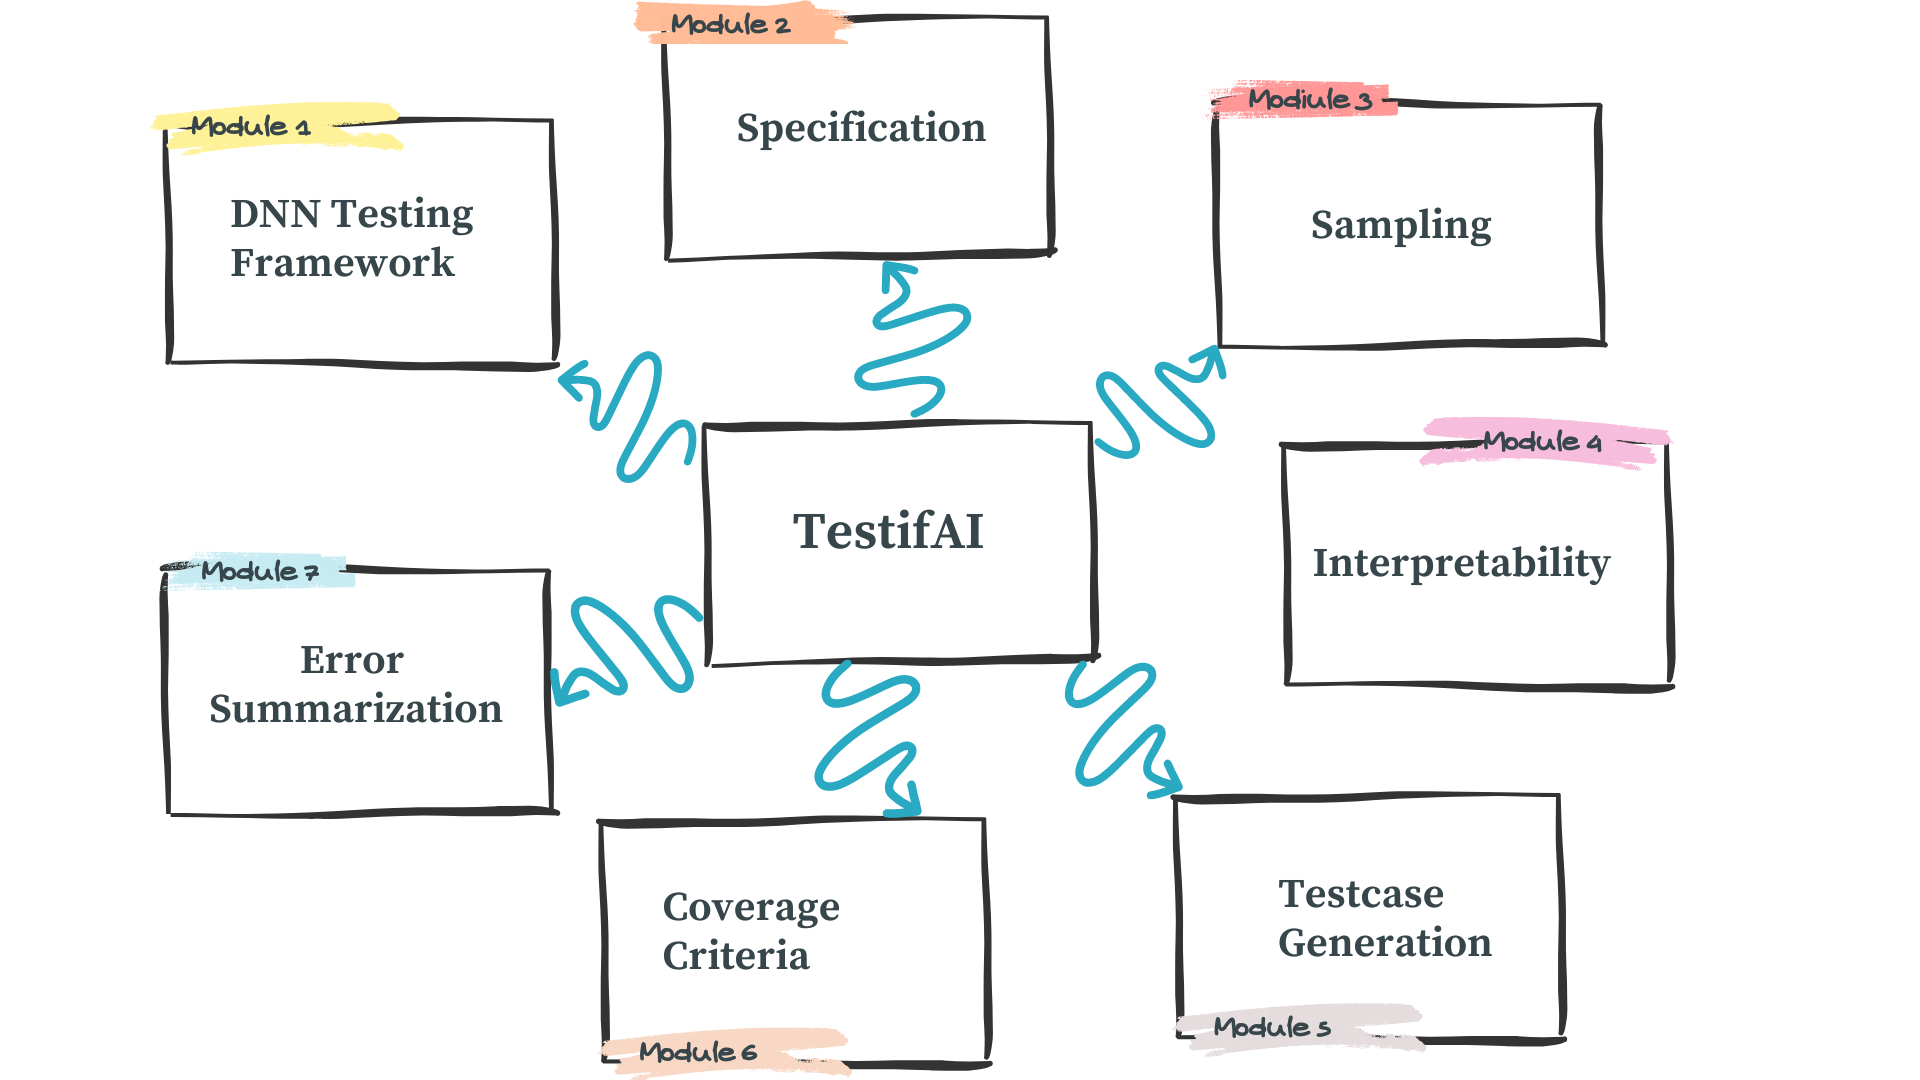
\includegraphics[width=\linewidth]{researchareas.png}
  \caption{Research Modules}
  \label{fig:no_publish}
\end{figure}

\section{Mapping of Research Modules to Objectives}
The research is structured into seven distinct modules, each addressing a specific objective. Table \ref{table:modules} outlines the mapping of these research modules to their corresponding objectives discussed in Section \ref{Research Questions and Objectives}.

\begin{table}[ht]
  \centering
  \renewcommand{\arraystretch}{1.5} % Adjusts the row padding
  \begin{tabular}{|l|l|}
    \hline
    \rowcolor[HTML]{000000} 
    \multicolumn{1}{|c|}{\cellcolor[HTML]{000000}{\color[HTML]{FFFFFF} \textbf{Research Modules}}} & {\color[HTML]{FFFFFF} \textbf{Research Objectives}} \\ \hline
    {\color[HTML]{404040} DNN Testing Framework} & Obj1 \\ \hline
    {\color[HTML]{404040} Specification} & Obj2 \\ \hline
    {\color[HTML]{404040} Sampling} & Obj3 \\ \hline
    {\color[HTML]{404040} Interpretability} & Obj4 \\ \hline
    {\color[HTML]{404040} Testcase Generation} & Obj5 \\ \hline
    {\color[HTML]{404040} Coverage Criteria} & Obj6 \\ \hline
    Error Summarization & Obj7 \\ \hline
  \end{tabular}
  \caption{Mapping of Research Modules to Objectives}
  \label{table:modules}
\end{table}

These modules are further divided into specific tasks to streamline the research process:

\subsection{DNN Testing Framework (Module 1, M\textsubscript{Oct24} - M\textsubscript{Sep25}, 43\% completion)} \noindent This module focuses on developing a comprehensive testing framework for DNNs. So far, 43\% of the work is done, including designing the framework, identifying key components, and implementing methods like adversarial and semantic adversarial testcase generation. Previous methods, such as resampling and testcase generation is combined with new solutions like local and global coverage to create a functional pipeline. Next year, I will refine and integrate all components to complete the framework. I have divided it into subtasks. Let's discuss each one in detail.

\noindent \textbf{5.2.1.1 Literature review (M\textsubscript{Oct24} - M\textsubscript{Dec24}, 50\% completion)}\ I have reviewed 50\% of existing DNN testing methods and identified key requirements. Moving forward, I will continue to outline comprehensive testing needs based on further findings.

\noindent \textbf{5.2.1.2 Designing a conceptual framework (M\textsubscript{Oct24} - M\textsubscript{Nov24}, 80\% completion)}\ I have designed 80\% of the framework. I will automate the remaining 20\% of the framework flow according to specified requirements, starting in October 2024.

\noindent \textbf{5.2.1.3 Design local and global coverage flow (M\textsubscript{Oct24} - M\textsubscript{Dec24}, 80\% completion)}\ The design of the local and global coverage flow is 80\% complete. I will focus on gaining more proficiency in running multiple scenarios, models, and datasets, and implementing existing coverage metrics to validate my local and global coverage concept.

\noindent \textbf{5.2.1.4 Implementing the simple real life example to calculate local to global robustness (M\textsubscript{Oct24} - M\textsubscript{Nov24}, 70\% completion)}\ Implemented a simple real-life example to calculate local to global robustness, reaching 70\% completion. The remaining work involves running this example on different DNNs to test effectiveness and further validate the approach.

\noindent \textbf{5.2.1.5 Implement probabilistic logic programming to calculate global coverage with simple examples (M\textsubscript{Oct24} - M\textsubscript{Nov24}, 80\% completion)}\ Set clear criteria for calculating the global coverage. Successfully implemented ProbLog by running a few simple examples, such as an adder and detecting different weather conditions by assuming specifications. These examples were successfully executed using ProbLog. In the coming months, I will run more complex scenarios and datasets related to autonomous driving cars.

\noindent \textbf{5.2.1.6 Integrate probLog code with python code (M\textsubscript{Oct24} - M\textsubscript{Dec24}, 80\% completion)}\ I successfully integrated ProbLog syntax with Python for simple scenarios. In the future, I will focus on integrating it with more complex scenarios and optimizing the code for these complex scenarios.

\noindent \textbf{5.2.1.7 Apply framework to different datasets (M\textsubscript{Oct24} - M\textsubscript{Jun25}, 50\% completion)}\ I have applied the framework, which includes both existing and my proposed components, to the CIFAR, MNIST, and DAWN datasets, reaching 50\% completion. In the future, I will move to more complex datasets, such as those related to autonomous vehicles and other advanced scenarios.

\noindent \textbf{5.2.1.8 Implement existing criteria and integrate proposed coverage criteria (M\textsubscript{Nov24} - M\textsubscript{Jan25}, 40\% completion)}\ I have implemented proposed coverage criteria (local and global) on simple examples, reaching 40\% completion. In the future, I will also implement existing criteria to compare and validate the results of my proposed criteria.

\noindent \textbf{5.2.1.9 Implement and integrate test cases (M\textsubscript{Dec24} - M\textsubscript{March25}, 42\% completion)}\ Implemented various adversarial examples from literature, such as FGSM, BIM and DeepFool, etc., using Foolbox and Adversarial Toolbox library. Additionally, I have implemented semantic adversarial examples like rotation, brightness, noise, and blur using Python code, 42\% is completed. In the future, I will focus on automating these processes and integrating this module into the framework.

\noindent \textbf{5.2.1.10 Implement and integrate interpretability analysis to identify critical features (M\textsubscript{Oct24} - M\textsubscript{Dec24}, 42\% completion)}\ I have explored and applied interpretability techniques, specifically SHAP, to identify critical features in CIFAR and MNIST datasets, reaching 42\% completion. This approach is unique as most research focuses on using these techniques for defensive mechanisms against adversarial examples. In the future, I will explore additional interpretability techniques like LIME and investigate how to better utilize them for my framework, as interpretability is a vast domain with significant potential for enhancing my study.

\noindent \textbf{5.2.1.11 Develop and integrate efficient sampling approach (M\textsubscript{Jan25} - M\textsubscript{Mar25}, 40\% completion)}\ I have read several sampling techniques that are not commonly used by researchers for testing DNNs. I have identified techniques like Borderline SMOTE and ADASYN for finding and prioritize the corner cases, which are not typically used for this purpose in the literature. In the future, I will apply these techniques and develop improved methods for efficient sampling to identify more corner cases.

\noindent \textbf{5.2.1.12 Develop and integrate error summarization modules (M\textsubscript{June25} - M\textsubscript{Aug25}, 0\% completion)}\ I found no existing literature on this component. I have planned to develop a new method for detailed error summarization. This part has not been started yet and will be addressed at the end after implementing all other components.

\noindent \textbf{5.2.1.13 Integrate all developed techniques (M\textsubscript{Aug25} - M\textsubscript{Sep25}, 0\% completion)}\ After working on individual components, I will integrate all components to work automatically within the framework. I will also apply existing methods of different literature papers to validate my proposed framework.


\noindent \textbf{5.2.1.14 Generate results on different datasets and make scenarios to validate this framework (M\textsubscript{Aug25} - M\textsubscript{Sep25}, 35\% completion)}\ Currently working with CIFAR, DAWN, and MNIST datasets, reaching 35\% completion. In the future, I will work with more datasets to further validate the framework.


\subsection{Specification (Module 2, M\textsubscript{Jan25} - M\textsubscript{May25}, 0\% completion)} I have not yet addressed this module in terms of literature or practical work. I tried to find relevant papers, but no significant work focuses on this area. Currently, I assume specifications based on user requirements and perform experiments. In the future, I will automate this part to align the framework with user requirements. I divided this module into subtasks. Let's discuss each one.


\noindent \textbf{5.2.2.1 Read literature about how specification is specified in other systems (M\textsubscript{Jan25} - M\textsubscript{Apr25}, 0\% completion)}\ I plan to work on this in Jan25, after implementing other components of framework. This task will involve reading literature about how specifications are specified in other systems.

\noindent \textbf{5.2.2.2 Find a way to define specification (M\textsubscript{Mar25} - M\textsubscript{Apr25}, 0\% completion)}\ I plan to work on this from Mar25 to Apr25. I will investigate how specifications are defined in other systems, whether they use templates or specific criteria. Additionally, I will determine if I need a template or criteria to define specifications, and how users should provide these, whether in raw form or a specific format.

\noindent \textbf{5.2.2.3 How to pass specifications to ProbLog (M\textsubscript{Apr25} - M\textsubscript{May25}, 0\% completion)}\ I will explore methods to efficiently pass specifications to ProbLog. This includes examin the required format and steps needed for integration between the defined specifications and the ProbLog system.

\noindent \textbf{5.2.2.4 How to automatically change specifications into desired format of framework (M\textsubscript{Apr25} - M\textsubscript{May25}, 0\% completion)}\ I will work on automating the conversion of specifications into the desired format for the framework. This task involves developing a method to transform user-provided specifications into a format compatible with the proposed framework.



\subsection{Sampling (Module 3, M\textsubscript{Jan25} - M\textsubscript{Mar25}, 40\% completion)} Currently, I have achieved 40\% completion by implementing existing sampling techniques specifically for DNN testing. However, I have not explored these techniques in detail. The detailed examination is still pending. So far, I have only implemented these techniques to determine their feasibility, as there is limited research in this area. The module have been separated into subtasks. Let's go through them individually.

\noindent \textbf{5.2.3.1 Reading papers related to sampling techniques and identify gaps (M\textsubscript{Jan25} - M\textsubscript{Feb25}, 50\% completion)}\  I will read various papers related to sampling techniques and identify gaps and potential areas for improvement. This task is already 50\% complete, covering initial literature review and gap identification.

\noindent \textbf{5.2.3.2 Develop efficient sampling technique (M\textsubscript{Feb25} - M\textsubscript{Feb25}, 0\% completion)}\ After identifying gaps in existing techniques, I will develop my own efficient sampling technique specifically for DNN testing. This task aims to create methods that can identify corner cases and enhance overall sampling efficiency.

\noindent \textbf{5.2.3.3 Implement existing sampling techniques (M\textsubscript{Mar25} - M\textsubscript{Mar25}, 70\% completion)}\ I will implement existing sampling techniques, which is already 70\% complete. This involves further testing of these techniques to ensure they are effective for DNN testing.

\noindent \textbf{5.2.3.4 Automate sample generation according to specification (M\textsubscript{Mar25} - M\textsubscript{Mar25}, 0\% completion)}\ I will work on automating the sample generation process according to specified criteria. This task aims to create an efficient method for generating samples that meet the defined specifications.

\subsection{Interpretability (Module 4, M\textsubscript{Oct24} - M\textsubscript{Dec24}, 42\% completion)} This module focuses on applying interpretability techniques to DNNs. Currently, I have achieved 42\% completion by implementing specific methods like SHAP to identify critical features in datasets such as CIFAR and MNIST. Future work will include exploring additional interpretability techniques and further integrating these methods into the framework. Ihave organized it into subtasks. Let's delve into each one specifically.

\noindent \textbf{5.2.4.1 Literature review (M\textsubscript{Oct24} - M\textsubscript{Nov24}, 30\% completion)}\  I will conduct a literature review on interpretability techniques for DNNs. Specifically, I will focus on how to use these techniques to identify critical pixels for effective test case generation, an area that has not been widely explored.

\noindent \textbf{5.2.4.2 Implement SHAP tool (M\textsubscript{Oct24} - M\textsubscript{Nov24}, 100\% completion)}\ Successfully implemented the SHAP tool to identify critical features in DNNs. This task is 100\% complete, providing insights into which pixels are most important for generating effective test cases.

\noindent \textbf{5.2.4.3 Apply SHAP to identify important pixels (M\textsubscript{Oct24} - M\textsubscript{Nov24}, 80\% completion)}\ I have applied the SHAP tool to identify important pixels in DNNs, reaching 80\% completion. In the future, I will apply this technique to different scenarios and datasets to further validate its effectiveness.


\noindent \textbf{5.2.4.4 Explore other interpretability analysis techniques (M\textsubscript{Oct24} - M\textsubscript{Nov24}, 0\% completion)}\ I will explore other interpretability techniques, such as LIME, to identify key features that can guide the generation of optimal test cases for evaluating model robustness. This task is scheduled from M\textsubscript{Oct24} - M\textsubscript{Nov24}, with 0\% completion currently.


\noindent \textbf{5.2.4.5 Automate interpretability approach in test case generation module (M\textsubscript{Nov24} - M\textsubscript{Dec24}, 0\% completion)}\  I will automate the interpretability approach in the test case generation module. This task aims to integrate advanced interpretability techniques to identify critical features in the dataset, which will be used to create effective test cases.

\subsection{Testcase Generation (Module 5, M\textsubscript{Dec24} - M\textsubscript{Mar25}, 42\% completion)} This module focuses on generating test cases for DNNs. Currently, I have achieved 42\% completion by implementing various adversarial and semantic test case generation techniques. Future work will involve automating these processes and integrating them into the overall framework. The module is divided into subtasks. Let's review each one in detail

\noindent \textbf{5.2.5.1 Literature review (M\textsubscript{Dec24} - M\textsubscript{Feb25}, 50\% completion)}\ Conducted a literature review on test case generation techniques for DNNs, reaching 50\% completion. This task covered the period from M\textsubscript{1} to M\textsubscript{18}, identifying key methods and gaps in the current research.

\noindent \textbf{5.2.5.2 Exploring libraries for test case generation (M\textsubscript{Dec24} - M\textsubscript{Jan25}, 80\% completion)}\ Explored various libraries for test case generation, reaching 80\% completion. This involved evaluating tools and frameworks that can be utilized for generating test cases for DNNs.

\noindent \textbf{5.2.5.3 Implementing adversarial attacks and semantic adversarial test cases (M\textsubscript{Dec24} - M\textsubscript{Dec24}, 80\% completion)}\ I have implemented adversarial attacks and semantic adversarial test cases, reaching 80\% completion. This involved creating test cases that simulate real-world adversarial scenarios and environmental variations to evaluate the robustness of DNNs.

\noindent \textbf{5.2.5.4 Apply existing test case generation methods to benchmark datasets (M\textsubscript{Jan25} - M\textsubscript{Feb25}, 0\% completion)}\ I will apply existing test case generation methods to benchmark datasets and analyze the results. This task is scheduled from M\textsubscript{13} to M\textsubscript{14}, with 0\% completion currently.

\noindent \textbf{5.2.5.5 Automate proposed test generation module (M\textsubscript{Feb25} - M\textsubscript{Mar25}, 0\% completion)}\ From Feb25 to Mar25, I will work on automating the proposed test generation module. This task aims to develop a seamless and efficient process for generating test cases automatically based on the proposed methods.

\subsection{Coverage Criteria (Module 6, M\textsubscript{Nov24} - M\textsubscript{Jan25}, 40\% completion)} This module focuses on developing and implementing coverage criteria for DNN testing. Currently, I have achieved 40\% completion by identifying and partially implementing existing coverage criteria. Future work will involve refining these criteria and integrating them into the overall framework. I have broken this module into subtasks. Let's go over each one in detail.


\noindent \textbf{5.2.6.1 Literature review on coverage criteria (M\textsubscript{Nov24} - M\textsubscript{Dec24}, 40\% completion)}\ I have reviewed literature on coverage criteria and found that existing methods often focus on internal structures of DNNs, neglecting comprehensive coverage. I proposed new local and global coverage concepts, designed, and implemented them using CIFAR and MNIST datasets. Future work will focus on refining and applying these criteria to improve DNN testing coverage.


\noindent \textbf{5.2.6.1 Reading papers and identifying gaps (M\textsubscript{Nov24} - M\textsubscript{Dec24}, 80\% completion)}\ I have reviewed relevant literature on coverage criteria and identified that many existing methods focus mainly on the internal structures of DNNs. I proposed new local and global coverage criteria to address these gaps. The work completed includes reviewing the current methods and implementing the proposed criteria using CIFAR and MNIST datasets. Future efforts will be directed towards further development and application of these coverage criteria.


\noindent \textbf{5.2.6.3 Apply existing coverage criteria to benchmark datasets (M\textsubscript{Nov24} - M\textsubscript{Dec24}, 0\% completion)}\ I plan to apply existing coverage criteria to benchmark datasets like CIFAR and MNIST. This task will involve evaluating the effectiveness of these criteria to understand their performance and limitations. The analysis will help determine how well the current methods align with the proposed coverage concepts and provide insights for further refinement.

\noindent \textbf{5.2.6.4 Reading literature on probLog to understand its application in calculating DNN global coverage (M\textsubscript{Dec24} - M\textsubscript{Dec24}, 50\% completion)}\ I will review literature on ProbLog to understand its application for calculating global coverage in DNNs. This review will explore how ProbLog has been used for global coverage analysis, identifying gaps and opportunities for improvement in the context of deep neural networks.


\noindent \textbf{5.2.6.5 Understand the probLog language and editor (M\textsubscript{Nov24} - M\textsubscript{Jan25}, 70\% completion)}\ I have achieved a 70\% understanding of the ProbLog language and its editor, including basic rule definitions and query manipulations. Further efforts will focus on deepening this knowledge and mastering advanced features to effectively implement and refine ProbLog-based solutions for coverage criteria.


\noindent \textbf{5.2.6.6 Implementing and automating probLog for DNN coverage calculations (M\textsubscript{Dec24} - M\textsubscript{Jan25}, 0\% completion)}\ I will implement and automate ProbLog to calculate DNN coverage. This will involve integrating ProbLog with the framework and automating its use to ensure accurate and efficient coverage calculations.

\subsection{Error Summarization (Module 7, M\textsubscript{Jun25} - M\textsubscript{Aug25}, 0\% completion)}This module, starting in June 2025, will focus on developing methods for summarizing errors in DNN testing. It will involve creating a new approach for error analysis and summarization, following the completion of all previous modules. I have split the work into subtasks. Let's discuss them one by one.


\noindent \textbf{5.2.7.1 Find ways to properly summarize the counter examples (M\textsubscript{Jun25} - M\textsubscript{July25}, 0\% completion)}\ I will explore methods to effectively summarize counterexamples in DNN testing. This will involve identifying techniques for detailed error analysis and summarization to enhance understanding and improve the framework's robustness.

\noindent \textbf{5.2.7.2 Best visuals to represent errors report (M\textsubscript{July25} - M\textsubscript{Aug25}, 0\% completion)}\ I will identify and implement effective visualizations to represent error reports. This involves evaluating various visualization techniques to determine which best conveys error patterns and insights, enhancing the clarity and usefulness of error summaries

\noindent \textbf{5.2.7.3 Integrate error summarization module in framework (M\textsubscript{July25} - M\textsubscript{Aug25}, 0\% completion)}\ I will integrate the error summarization module into the existing framework. This will involve ensuring that the module works seamlessly with other components and effectively summarizes errors generated during testing, providing a comprehensive view of model performance and issues.

\section{Mapping of Research Milestones to Objectives}
This section outlines the key milestones in the research timeline.The planned milestones and their associated research objectives are detailed in Table \ref{table:milestones}. This table maps each milestone to the specific objectives it addresses, including major conferences, journal papers, and thesis-related activities.

\noindent \textbf{MS1: Conference 1} \
I will present initial research findings and theoretical contributions at the first conference, focusing on early results and their implications.

\noindent \textbf{MS2: Conference 2} \
I will showcase refined results and new insights at the second conference. This presentation will highlight advancements in methodology and preliminary data analysis.

\noindent \textbf{MS3: Journal 1} \
I will publish a detailed research paper in a peer-reviewed journal, documenting significant findings and contributions to the field.

\noindent \textbf{MS4: Conference 3} \
I will present further research progress and innovations at the third conference, focusing on advanced techniques and expanded data sets.

\noindent \textbf{MS5: Conference 4} \
I will deliver a presentation on the latest developments and comprehensive results at the fourth conference, emphasizing contributions to current research trends.

\noindent \textbf{MS6: Journal 2 } \
I will submit and publish a follow-up paper in a second peer-reviewed journal, detailing additional findings and improvements from recent research.

\noindent \textbf{MS7: Thesis Writing } \
I will draft the thesis, integrating all research milestones, methodologies, and results. This will involve organizing and presenting comprehensive findings.

\noindent \textbf{MS8: Thesis Submission} \
I will submit the finalized thesis to the academic committee for review, incorporating feedback and ensuring that all research objectives and contributions are documented.

\noindent \textbf{MS9: Defense and Final Submission} \
I will prepare for and conduct the thesis defense, make final revisions based on feedback, and submit the final version of the thesis, completing the research project.

\begin{table*}[ht]
  \centering
  \renewcommand{\arraystretch}{1.5} 
  \resizebox{\textwidth}{!}{%
    \begin{tabular}{|l|l|}
      \hline
      \rowcolor[HTML]{000000} 
      \multicolumn{1}{|c|}{\cellcolor[HTML]{000000}{\color[HTML]{FFFFFF} \textbf{Milestones}}} & {\color[HTML]{FFFFFF} \textbf{Research Objectives}} \\ \hline
      {\color[HTML]{404040} Conference 1 (EuroML Conf 2025)} & Obj1, 4, 6 \\ \hline
      {\color[HTML]{404040} Conference 2 (ICSE 2025)} & Obj2 \\ \hline
      {\color[HTML]{404040} Journal paper 1 (Neural Networks)} & Obj1, 2, 4, 6 \\ \hline
      {\color[HTML]{404040} Conference 3 (ASE 2025)} & Obj3 \\ \hline
      {\color[HTML]{404040} Conference 4 (ICST 2025)} & Obj7 \\ \hline
      {\color[HTML]{404040} Journal paper 2 (IEEE Transaction on Software Engineering)} & Obj1, 2, 3, 7 \\ \hline
      {\color[HTML]{404040} Thesis writing} & compile and synthesize research findings  \\ \hline
      {\color[HTML]{404040} Thesis submission} & finalize and submit the complete thesis  \\ \hline
      {\color[HTML]{404040} Defense and final submission} & present research, address feedback, and submit final version\\ \hline
    \end{tabular}
  }
  \caption{Mapping of Research Milestones to Objectives}
  \label{table:milestones}
\end{table*}


\section{Gantt Chart for Task-Wise Completion}
The Gantt chart provides a clear timeline and progress overview for the research project. Modules, such as Module 1 (M1), Module 2 (M2), and Module 3 (M3), are depicted with color-coded bars to indicate their progress. The dark blue bars represent the percentage of work completed within each module, reflecting the overall progress. In contrast, black lines show the completion status for each Module. Tasks following the M1,2,3..7, are represented by blue lines. The sky blue bars indicate the percentage of completion for these tasks, while the light blue bars represent the remaining portion that is still pending. Milestones, such as Conference paper 1 (MS1), are marked with red circles, highlighting key achievements and deadlines. This color-coding effectively communicates the status and progress of various tasks and milestones throughout the project.

\hspace{-3.5cm}
\begin{ganttchart}[
  y unit chart=0.6cm,
  x unit=0.023cm,
  vgrid={*1{draw=none}, *1{draw=black!10}}, % Reduce vertical grid lines
  hgrid={*1{draw=black!20}}, % Reduce horizontal grid lines
  time slot format=isodate,
  title/.append style={fill=none, draw=black},
  title label font=\bfseries\footnotesize\color{black},
  bar/.append style={draw=none, fill=barblue},
  bar incomplete/.append style={fill=barblue!50},
  bar label font=\bfseries\footnotesize\color{black},
  group incomplete/.append style={fill=groupblue},
  group left shift=0,
  group right shift=0,
  group height=.4,
  group peaks tip position=0,
  group label node/.append style={left=.5cm},
  group progress label font=\bfseries\small,
  link/.append style={-latex, line width=1.5pt, linkred},
  link label font=\scriptsize\bfseries,
  link label node/.append style={below left=-2pt and 4pt},
  milestone/.append style={shape=circle, fill=none},
  milestone label font=\bfseries\footnotesize\color{red},
  milestone label node/.append style={left=5mm, above left=-5mm and 0mm}
]{2024-10-01}{2026-11-30}
\gantttitlecalendar{year, month=shortname} \\

% Module 1: DNN Testing Framework
\ganttgroup[progress=43]{M1}{2024-10-01}{2025-9-29} \\
\ganttbar[progress=50]{5.2.1.1}{2024-10-01}{2024-12-28}\\ % Literature review (M1-M5)
\ganttbar[progress=80]{5.2.1.2}{2024-10-01}{2024-11-30}\\ % Designing a conceptual framework (M8-M12)
\ganttbar[progress=80]{5.2.1.3}{2024-10-01}{2024-12-31} \\% Design local and global coverage flow (M8-M10)
\ganttbar[progress=70]{5.2.1.4}{2024-10-01}{2024-11-31}\\ % Implementing the Simple real life Example (M8-M10)
\ganttbar[progress=80]{5.2.1.5}{2024-10-01}{2024-11-30} \\% Implementing ProbLog for calculating global robustness (M9-M11)
\ganttbar[progress=80]{5.2.1.6}{2024-10-01}{2024-12-30} \\% Integrate ProbLog code with python code (M9-M11)
\ganttbar[progress=50]{5.2.1.7}{2024-10-01}{2025-6-31} \\% Applying the framework to different datset
\ganttbar[progress=40]{5.2.1.8}{2024-11-01}{2025-1-30} \\% Implement exisiting criterias and integrate proposed coverage criteria 

\ganttbar[progress=42]{5.2.1.9}{2024-12-01}{2025-3-3} \\% Implement and integrate testcases 
\ganttbar[progress=42]{5.2.1.10}{2024-10-01}{2024-12-31} \\% Implement and integrate interpratability analysis to identofy critical features


% Milestone MS1 with red dot
\ganttmilestone[
  milestone/.append style={shape=circle, fill=red, minimum size=3mm},
  milestone label font=\bfseries\footnotesize\color{black},
  milestone label node/.append style={right=20mm, yshift=0mm}
]{Conference paper 1(MS1)}{2024-12-15}\\

\ganttbar[progress=40]{5.2.1.11}{2025-1-01}{2025-3-30} \\% Develop and integrate efficient sampling approach
\ganttbar[progress=0]{5.2.1.12}{2025-1-01}{2025-5-30} \\% Develop and integrate specifcation templates
\ganttbar[progress=0]{5.2.1.13}{2025-6-01}{2025-8-30} \\% Develop and integrate error summarzation modules
\ganttbar[progress=0]{5.2.1.14}{2025-8-01}{2025-9-30} \\% Integrate all developed techniques
\ganttbar[progress=35]{5.2.1.15}{2025-8-01}{2025-9-10} \\% Generate results on different datasets  and make scenarios to validate this framework.


% Module 2: Specification
\ganttgroup[progress=0]{M2} {2025-01-01}{2025-5-30} \\
\ganttbar[progress=0]{5.2.2.1}{2025-01-01}{2025-04-31} \\% Read literature about how specification specified in other systems
\ganttbar[progress=0]{5.2.2.1}{2025-03-01}{2025-04-31} \\% Find a way to define specification (M20-M23)
\ganttbar[progress=0]{5.2.2.2}{2025-04-01}{2025-05-31} \\% How to pass specifications to ProbLog (M20-M23)
\ganttbar[progress=0]{5.2.2.3}{2025-04-01}{2025-05-1}\\ % How to automatically change specifications into desired format of framework

% \ganttmilestone{MS2}{2025-05-30}\\

% \ganttmilestone[inline]{\tikz \node[shape=circle, fill=red, minimum size=3mm, inner sep=0pt] {};\ MS1}{2025-05-30}\\

\ganttmilestone[
  milestone/.append style={shape=circle, fill=red, minimum size=3mm},
  milestone label font=\bfseries\footnotesize\color{black},
  milestone label node/.append style={right=60mm, yshift=0mm}
]{Conference paper 2(MS2)}{2025-05-30}\\

\ganttmilestone[
  milestone/.append style={shape=circle, fill=red, minimum size=3mm},
  milestone label font=\bfseries\footnotesize\color{black},
  milestone label node/.append style={right=29mm, yshift=0mm}
]{Journal paper 1(MS3)}{2025-1-30}\\

  % % Module 3: Sampling

% \ganttmilestone{MS4}{2025-1-30}\\
\ganttgroup[progress=40]{M3}{2025-1-1}{2025-03-30} \\
\ganttbar[progress=50]{5.2.3.1}{2025-1-1}{2025-02-15}\\ % Reading Papers Related to Sampling Techniques and Identify Gaps (M9-M10)
\ganttbar[progress=0]{5.2.3.2}{2025-2-15}{2025-02-30} \\% Develop Efficient Sampling Technique (M10-M12)
\ganttbar[progress=70]{5.2.3.3}{2025-3-01}{2025-3-10} \\% Implement Existing Sampling Techniques (M9-M10)
\ganttbar[progress=0]{5.2.3.4}{2025-3-01}{2025-03-30} \\% Automate sampling according to specification
% \ganttmilestone{MS4}{2025-3-15}\\
\ganttmilestone[
  milestone/.append style={shape=circle, fill=red, minimum size=3mm},
  milestone label font=\bfseries\footnotesize\color{black},
  milestone label node/.append style={right=40mm, yshift=0mm}
]{Conference paper 3(MS4)}{2025-3-15}\\


\end{ganttchart}
\newpage
\hspace{-3.5cm}
\begin{ganttchart}[
  y unit chart=0.6cm,
  x unit=0.023cm,
  vgrid={*1{draw=none}, *1{draw=black!10}}, % Reduce vertical grid lines
  hgrid={*1{draw=black!20}}, % Reduce horizontal grid lines
  time slot format=isodate,
  title/.append style={fill=none, draw=black},
  title label font=\bfseries\footnotesize\color{black},
  bar/.append style={draw=none, fill=barblue},
  bar incomplete/.append style={fill=barblue!50},
  bar label font=\bfseries\footnotesize\color{black},
  group incomplete/.append style={fill=groupblue},
  group left shift=0,
  group right shift=0,
  group height=.4,
  group peaks tip position=0,
  group label node/.append style={left=.5cm},
  group progress label font=\bfseries\small,
  link/.append style={-latex, line width=1.5pt, linkred},
  link label font=\scriptsize\bfseries,
  link label node/.append style={below left=-2pt and 0pt},
  milestone/.append style={shape=circle, fill=red, minimum size=5mm},
  milestone label font=\bfseries\footnotesize\color{red},
  milestone label node/.append style={left=5mm, above left=-5mm and 0mm}
]{2024-10-01}{2026-11-30}
  \gantttitlecalendar{year, month=shortname} \\


  % % Module 4: Interpretability 2024-10-01}{2024-12-31}
  \ganttgroup[progress=42]{M4}{2024-10-01}{2024-12-31} \\
  \ganttbar[progress=30]{5.2.4.1}{2024-10-01}{2024-11-30}\\ % Literature Review (M4-M24)
  \ganttbar[progress=100]{5.2.4.2}{2024-10-01}{2024-11-31}\\ % Implementation of SHAP Tool (M4-M6)
  \ganttbar[progress=80]{5.2.4.3}{2024-10-01}{2024-11-31}\\ % Applying SHAP to Identify Important Pixels (M4-M5)
  \ganttbar[progress=0]{5.2.4.4}{2024-10-15}{2024-11-30}\\ % Explore Other Interpretability Analysis Techniques (M15-M17)
  \ganttbar[progress=0]{5.2.4.5}{2024-11-01}{2024-12-30}\\ 
  % Automate Interpretability Approach in Test Case Generation Module (M16-M17)



% Module 5: Testcase Generation {2024-12-01}{2025-3-3} 
\ganttgroup[progress=42]{M5}{2024-12-01}{2025-03-03} \\
\ganttbar[progress=50]{5.2.5.1}{2024-12-01}{2025-02-31}\\ % Literature Review (M1-M18)
\ganttbar[progress=80]{5.2.5.2}{2024-12-01}{2025-01-1}\\ % Exploring Libraries for Test Case Generation (M1-M2)
\ganttbar[progress=80]{5.2.5.3}{2024-12-01}{2024-12-31}\\ % Implementing Adversarial Attacks and Semantic Adversarial Test Cases (M3-M4)
\ganttbar[progress=0]{5.2.5.4}{2025-1-01}{2025-02-30}\\ % Apply Existing Test Case Generation Methods to Benchmark Datasets (M13-M14)
\ganttbar[progress=0]{5.2.5.5}{2025-2-01}{2025-03-30}\\ % Automate Proposed Test Generation Module (M15-M16)

% Module 6: Coverage Criteria {2024-11-01}{2025-1-30} 
\ganttgroup[progress=40]{M6}{2024-11-01}{2025-1-30} \\
\ganttbar[progress=80]{5.2.6.1}{2024-11-01}{2024-12-1}\\ % Reading Papers and Identifying Gaps (M6-M9)
\ganttbar[progress=0]{5.2.6.2}{2024-11-01}{2024-12-30}\\ % Apply Existing Coverage Criteria to Benchmark Datasets (M13-M14)
\ganttbar[progress=50]{5.2.6.3}{2024-12-01}{2024-12-31}\\ % Reading Literature on ProbLog to Understand its Application in Calculating DNN Global Coverage

\ganttbar[progress=70]{5.2.6.4}{2024-11-01}{2025-1-30} \\% Understand the Problog Language and Editor (M9-M10)
\ganttbar[progress=0]{5.2.6.5}{2024-12-01}{2025-1-30}\\ % Implementing and Automating ProbLog for DNN Coverage Calculations


% Module 7: Error Summarization {2025-6-01}{2025-8-30}
\ganttgroup[progress=0]{M7}{2025-6-01}{2025-08-30} \\
\ganttbar[progress=0]{5.2.7.1}{2025-06-01}{2025-07-31}\\ % Find Ways to Properly Summarize the Counter Examples (M17-M18)
\ganttbar[progress=0]{5.2.7.2}{2025-7-01}{2025-08-30} \\% Best Visuals to Represent Errors Report (M18-M20)
\ganttbar[progress=0]{5.2.7.3}{2025-7-01}{2025-08-30}\\ % Integrate Error Summarization Module in Framework (M20-M21)

\ganttmilestone[
  milestone/.append style={shape=circle, fill=red, minimum size=3mm},
  milestone label font=\bfseries\footnotesize\color{black},
  milestone label node/.append style={right=120mm, yshift=0mm}
]{Conference paper 4(MS5)}{2026-02-30}\\

\ganttmilestone[
  milestone/.append style={shape=circle, fill=red, minimum size=3mm},
  milestone label font=\bfseries\footnotesize\color{black},
  milestone label node/.append style={right=143mm, yshift=0mm}
]{Journal paper 2(MS6)}{2026-06-1}\\


% \ganttmilestone{MS5}{2025-08-30}\\
% \ganttmilestone{MS4}{2025-09-1}\\

% \ganttbar[progress=20]{\textcolor{red}{MS7}}{2024-10-01}{2026-05-30} \\
 \ganttbar[progress=20]{MS7}{2024-10-01}{2026-05-30} \\
\ganttmilestone[
  milestone/.append style={shape=circle, fill=red, minimum size=3mm},
  milestone label font=\bfseries\footnotesize\color{black},
  milestone label node/.append style={right=110mm, yshift=0mm}
]{Thesis submission(MS8)}{2026-7-30}\\
\ganttmilestone[
  milestone/.append style={shape=circle, fill=red, minimum size=3mm},
  milestone label font=\bfseries\footnotesize\color{black},
  milestone label node/.append style={right=112mm, yshift=0mm}
]{Defense and final submission(MS9)}{2026-10-30}\\


% \ganttmilestone{MS8}{2026-7-30}\\
% % \ganttbar[progress=0]{MS9}{2026-7-01}{2026-10-30} \\
% \ganttmilestone{MS9}{2026-10-30}\\
\end{ganttchart}
% \end{landscape}
% }
